\documentclass[12pt,a4paper]{article}
\usepackage{inverba}

\newcommand{\userName}{Cullyn Newman} 
\newcommand{\class}{[Subject]} 
\newcommand{\institution}{[Institution]} 
\newcommand{\theTitle}{\color{B-Cold} [Subject Title]}

\begin{document}
%%%%%%%%%%%%%%%%%%%%%%%%%%%%%%%%%%%%%%%%%%%%%%%%%%%%%%%%%%%%%%%%%%%%%
\tableofcontents
\cleardoublepage
\fancyhead{}
\fancyhead[R]{\hyperlink{home}{\nouppercase\leftmark}}
%%%%%%%%%%%%%%%%%%%%%%%%%%%%%%%%%%%%%%%%%%%%%%%%%%%%%%%%%%%%%%%%%%%%%
\clearpage
\section*{Week 6}\phantomsection
\addcontentsline{toc}{section}{\textbf{Week 6}}
\fancyhead[R]{\hyperlink{home}{Week 6}}

\fancyhead[L]{\hyperlink{home}{Monday, November 2}}
\subsection{Monday, November 2}
\begin{enumerate}
    {\color{G-Moon}\item What is the name of the following molecule?
    
    \chemfig{*6((-\ch{Br})---(-\ch{CH3})-(-\ch{Cl})--)}
    \vspace*{10pt}
    }
        \begin{itemize}
            \item {\color{o-Sun}\textbf{4-bromo-1-chloro-2-metyhlcyclohexane}}
            \begin{itemize}
                \item Lowest sum and alphabetically ordered.
            \end{itemize}
        \end{itemize}
    {\color{G-Moon}\item What is the definition of a molecular conformation?}
        \begin{itemize}
            \item {\color{o-Sun}\textbf{A geometric arrangement in space of a molecule that has a low energy pathway to rearrangement}}
            \begin{itemize}
                \item \textbf{Conformations}: the variety of possible three-dimensional shapes of a molecule that are interchangeable by low energy pathways.
                    \begin{itemize}
                        \item Conformations vary in potential energy.
                        \item Changes due to rotation about $\sigma$ bonds.
                    \end{itemize}
            \end{itemize}
        \end{itemize}
    {\color{G-Moon}\item What is the following molecule?
    
    (The package that draws newman projections is not compatable with the font I use... working on a fix, but can't draw them at the moment)
    }
        \begin{itemize}
            \item {\color{o-Sun}\textbf{pentane}}
            \begin{itemize}
                \item Front portion has 3 carbons in the chain: \ch{CH3} (1), \ch{CH2} (2), and the \ang{4} carbon (3) in the center.
                \item The circle represents the $\sigma$ bond between the carbon behind it, so thats (4).
                \item The methyl (\ch{CH3}) on the back portion is (5).
            \end{itemize}
        \end{itemize}
        \newpage
    {\color{G-Moon}\item For the molecule in the previous question, which conformer is the gauche form of the molecule?}
        \begin{itemize}
            \item {\color{o-Sun}\textbf{choice 1}}
            \item Can't draw newman projections currently; it's broken... but here's this lame screenshot:
            
            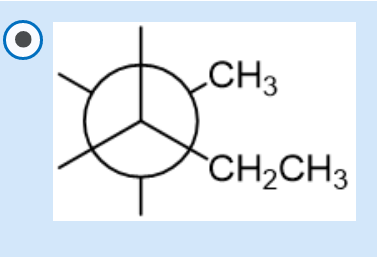
\includegraphics[scale=0.3]{images/newman1.png}
            \begin{itemize}
                \item \textbf{Gauche interaction}: unfavorable intereaction between groups, causing an increases in energy due to electron cloud repulsion.
                \item Gauche intereaction is a type of steric intereactions present at \(\approx\pm\ang{60}\) the next eclipsed conformation. 
                \end{itemize}
        \end{itemize}
    {\color{G-Moon}\item For the same molecule, which conformation corresponds to the most stable form?}
        \begin{itemize}
            \item {\color{o-Sun}\textbf{pick number 1 m'lord}}
            \item ugggghhhhhhhhhhhhhh so ugly :(
            
            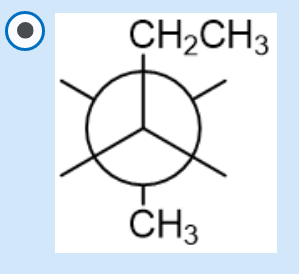
\includegraphics[scale=0.3]{images/newman2.png}
            \begin{itemize}
                \item Other forms represent an eclipsed form and the gauche interaction, both which increases potential energy due to increased torsional strain.
                \item More notes for reference:
                    \begin{itemize}
                        \item \textbf{dihedral (torsional) angle}: the angle between substituents of front and back carbons as the $\sigma$ bonds rotates.
                        \item \textbf{Staggered conformation}: {\color{o-Sun}lowest energy} conformation, when two substituents are at maximum dihedral angle from each other.
                        \item \textbf{Eclipsed conformation}: the {\color{o-Sun}highest energy} conformation, when two substituents are at the minimum dihedral angle from each other.
                    \end{itemize}
            \end{itemize}
        \end{itemize}
    \newpage
    {\color{G-Moon}\item For which molecule will the energy of conversion (E\(_{\text{act}}\)) be the greatest?}
        \begin{itemize}
            \item {\color{o-Sun}\textbf{butane}}
            \begin{itemize}
                \item I don't really know what E\(_{\text{act}}\) is, but I assume it's the energy required to go through the interchangeable pathway.
                \item Costs of butane: 
                    \begin{itemize}
                        \item \SI{19}{kJ\per\mole} (eclipsed with methyl overlap; once) 
                        \item \SI{16}{kJ\per\mole} (eclipsed, no methyl, but with gauche; twice)
                        \item \SI{3.8}{kJ\per\mole} (gauche only; twice)
                    \end{itemize}
                \item I'm not sure if you add them up or just take max, but either way butane has the greatest out of ethane, propane, and methane.
            \end{itemize}
        \end{itemize}
    {\color{G-Moon}\item Why is the cyclohexane ring more stable than rings of other sizes?
    \begin{itemize}
        \item the bond angles are all nearly \ang{109.5}
        \item the ring strain is at a minimum
        \item the overlap of the sp\(^{3}\) hybrid orbitals is at a maximum
    \end{itemize}}
        \begin{itemize}
            \item {\color{o-Sun}\textbf{all of the above}}
            \begin{itemize}
                \item This is true in the most stable, chair conformaions at least.
            \end{itemize}
        \end{itemize}
    {\color{G-Moon}\item Why can't the cyclobutane ring be square planar?}
        \begin{itemize}
            \item {\color{o-Sun}\textbf{the 2s orbitals wouldn't overlap well} OR the sp\(^{3}\) orbitals wouldn't overlap well}
            \begin{itemize}
                \item Cyclobutane adopts a slightly puckered conformation in order to reduce angle strain (and eclipsed H)... which I now assume is the because 2s orbitals after getting the question wrong twice.
            \end{itemize}
        \end{itemize}
    {\color{G-Moon}\item In the cartoon picture shown below, who's on the chair and who's on the boat forms of cyclohexane?}
        \begin{itemize}
            \item {\color{o-Sun}\textbf{she's on the chair and he's on the boat}}
            \begin{itemize}
                \item Hmmmmmmmmmmmm....
            \end{itemize}
        \end{itemize}
    {\color{G-Moon}\item What is the total energy for the cyclohexane ring flipping process?}
        \begin{itemize}
            \item {\color{o-Sun}\textbf{12.1}}
            \begin{itemize}
                \item Appears to be just the cost of the first flip to the half chair.
                \item Can't seem to find good explanation to why, however.
            \end{itemize}
        \end{itemize}
\end{enumerate}


\end{document}